Are sales trends for two industrial products related? The two time series objects described below contain Sales of chemicals and allied products; and Sales of motor vehicles and parts, in the U.S. for each month from Jan. 1971 to Dec. 1991. File is petr.txt. \\

\noindent You should analyze the data in the "chemicals" time series and the "vehicles" time series and write a report to address such questions as:
\begin{enumerate}[label=(\roman*)]
    \item What trend model(s) best capture the trends in sales of chemicals over time?
    \item What trend model(s) best capture the trends in sales of vehicles over time? Once the trend
has been accounted for, what can you say about the behavior of the detrended data, for both
models? Can either the original time series or the detrended series be described using any
common models?
    \item For the various models you tried, assess their fit. Can any transformations improve the
fit? Is there any apparent association between chemical sales and vehicle sales over time? If so,
describe the association.
    \item Make conclusions that relate to how the sales amounts (for both chemicals and vehicles)
change, both long-term over the observed period of years, and in terms of patterns of month-
to-month variation.
\end{enumerate}

\subsection{R Code}
\lstinputlisting[language=R]{Codes/Midterm_2_P3.R}
\subsection{Results}
\begin{enumerate}[label=(\roman*)]
    \item \begin{minipage}[!h]{0.9\linewidth}
    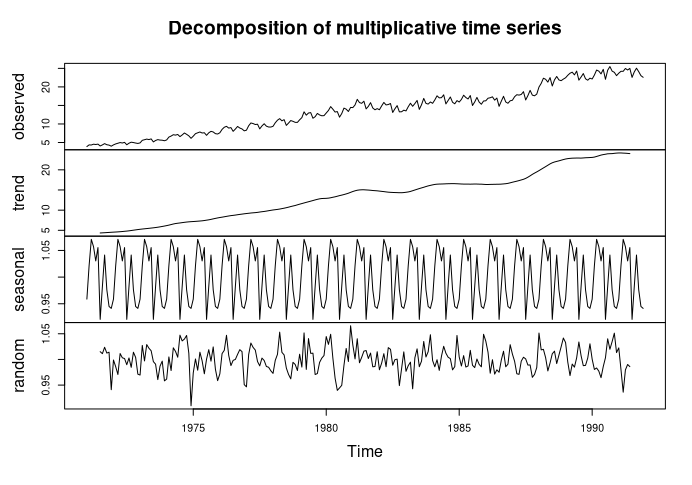
\includegraphics[width=\linewidth]{Images/P3/Chemicals_Plot.png}
    \captionof{figure}[Decomposition of the Chemicals data.]{Decomposition of the Chemicals data shows that both trend and seasonality are present.}
    \end{minipage}
    
    \item \begin{minipage}[!h]{0.9\linewidth}
    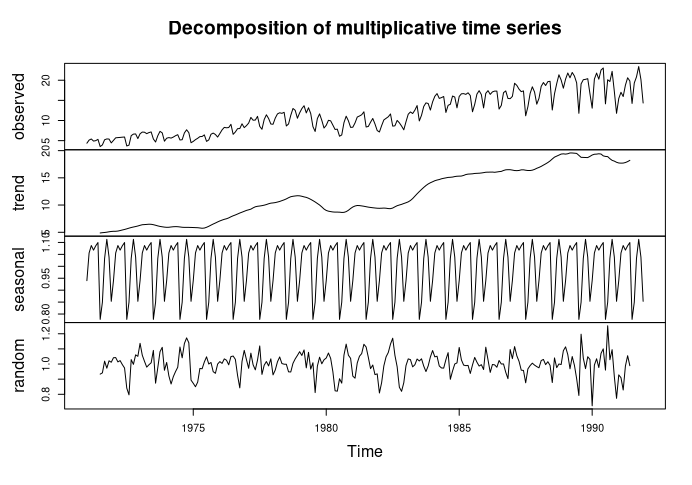
\includegraphics[width=\linewidth]{Images/P3/Vehicles_Plot.png}
    \captionof{figure}[Decomposition of the Vehicles data.]{Decomposition of the Vehicles data.}
    \end{minipage} \\
    Here, we again observe that the data exhibit both trend and seasonality. Nevertheless, in both the cases, we check their stationarity.
    \small\begin{block}
> adf.test(chemicals.data)

Augmented Dickey-Fuller Test
data:  chemicals.data
Dickey-Fuller = -3.0203, Lag order = 6, p-value = 0.1462
alternative hypothesis: stationary

> adf.test(vehicles.data)
Augmented Dickey-Fuller Test
data:  vehicles.data
Dickey-Fuller = -2.9112, Lag order = 6, p-value = 0.1921
alternative hypothesis: stationary
\end{block}
\normalsize The augmented Dickey-Fuller tests for both the datasets fail to reject the null hypothesis, and hence, these time series data are not stationary. Therefore, we detrend (also remove seasonality) these, and the time series plots are shown in Fig \ref{fig:diff_plots}.
\begin{figure}[!htb]
    \centering
    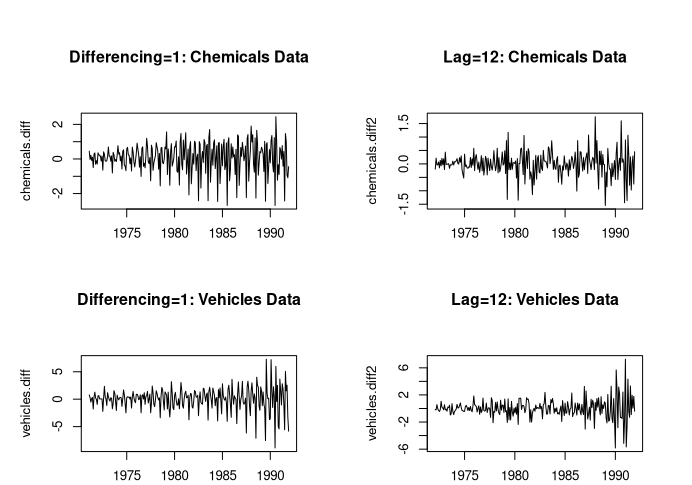
\includegraphics[width=\linewidth]{Images/P3/Diff_Plots.png}
    \caption[Time series plots of the detrended data.]{Time series plots of the detrended data. At first, the linear trend is removed using the first differences. Then the seasonality of the differenced data is removed by setting lag=12 as we deal with monthly data here.}
    \label{fig:diff_plots}
\end{figure}

The visual observation of the final detrended (Fig \ref{fig:diff_plots}) data show that both the time series have become stationary. We further test this using the augmented Dickey-Fuller test which confirms that we have achieved stationarity.
\small\begin{block}
> adf.test(chemicals.diff2)

Augmented Dickey-Fuller Test
data:  chemicals.diff2
Dickey-Fuller = -5.6096, Lag order = 6, p-value = 0.01
alternative hypothesis: stationary

> adf.test(vehicles.diff2)

Augmented Dickey-Fuller Test
data:  vehicles.diff2
Dickey-Fuller = -7.1672, Lag order = 6, p-value = 0.01
alternative hypothesis: stationary
\end{block}
\normalsize Here, the original data can be described as a harmonic model with increasing trend. However, for the detrended data, we can calculate the ACF, PACF, and EACF to get an idea about the order of the ARIMA process.  
\item Initally, we check the result of the harmonic model fit over the original data. \small\begin{block}
Call:
lm(formula = chemicals.data ~ har + time(chemicals.data))

Residuals:
    Min      1Q  Median      3Q     Max 
-4.0447 -0.5332  0.0430  0.6677  3.0799 

Coefficients:
                       Estimate Std. Error t value Pr(>|t|)    
(Intercept)          -1.951e+03  2.365e+01 -82.478  < 2e-16 ***
harcos(2*pi*t)       -9.564e-02  1.023e-01  -0.935    0.351    
harsin(2*pi*t)        5.420e-01  1.023e-01   5.297  2.6e-07 ***
time(chemicals.data)  9.913e-01  1.194e-02  83.058  < 2e-16 ***
---
Signif. codes:  0 ‘***’ 0.001 ‘**’ 0.01 ‘*’ 0.05 ‘.’ 0.1 ‘ ’ 1

Residual standard error: 1.148 on 248 degrees of freedom
Multiple R-squared:  0.9653,	Adjusted R-squared:  0.9649 
F-statistic:  2302 on 3 and 248 DF,  p-value: < 2.2e-16

Call:
lm(formula = vehicles.data ~ har + time(vehicles.data))

Residuals:
    Min      1Q  Median      3Q     Max 
-7.0874 -1.3989  0.3886  1.5226  4.5814 

Coefficients:
                      Estimate Std. Error t value Pr(>|t|)    
(Intercept)         -1.499e+03  4.476e+01 -33.497  < 2e-16 ***
harcos(2*pi*t)       2.120e-01  1.935e-01   1.095  0.27449    
harsin(2*pi*t)       5.378e-01  1.936e-01   2.777  0.00591 ** 
time(vehicles.data)  7.626e-01  2.259e-02  33.760  < 2e-16 ***
---
Signif. codes:  0 ‘***’ 0.001 ‘**’ 0.01 ‘*’ 0.05 ‘.’ 0.1 ‘ ’ 1

Residual standard error: 2.172 on 248 degrees of freedom
Multiple R-squared:  0.8217,	Adjusted R-squared:  0.8195 
F-statistic: 380.9 on 3 and 248 DF,  p-value: < 2.2e-16
\end{block}
\normalsize While the R\textsuperscript{2} is good for both cases, the residual standard error is quite high along with the F-statistic. The model fits for both the original datasets are depicted in Fig \ref{fig:harmonic_fit}. 
\begin{figure}[!htb]
    \centering
    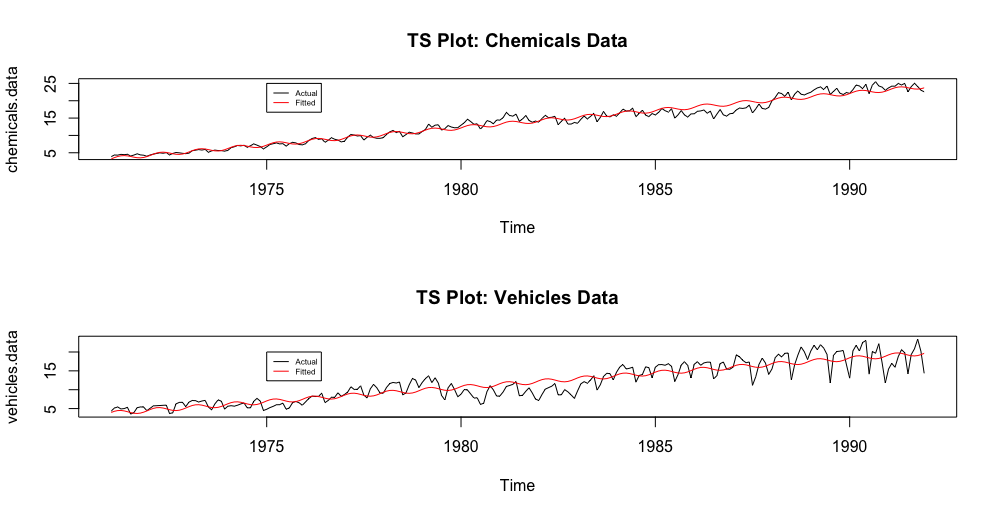
\includegraphics[width=\linewidth]{Images/P3/LFits_Original.png}
    \caption[Fitting a harmonic model with linear trend over the original data.]{Fitting a harmonic model with linear trend over the original data. We see that this model somewhat matches the time series pattern but misses out a lot. Increasing the number of harmonic pairs better fits the model but could lead to possible overfitting and results in a non-parsimonious model.}
    \label{fig:harmonic_fit}
\end{figure}
We now perform the residual diagnostics of the fit. 
\begin{figure}[!htb]
    \centering
    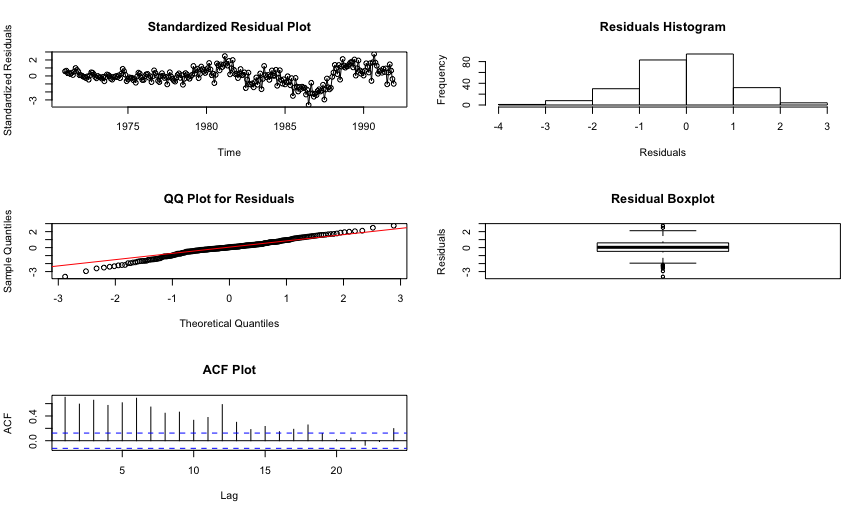
\includegraphics[width=\linewidth]{Images/P3/LFit_Res_Chem.png}
    \caption[Residual diagnostics of the harmonic fit over the original Chemicals data.]{Residual diagnostics of the harmonic fit over the original Chemicals data. Here, we see the non-normality of the residuals.}
    \label{fig:res_chem_har}
\end{figure}
\begin{figure}[!htb]
    \centering
    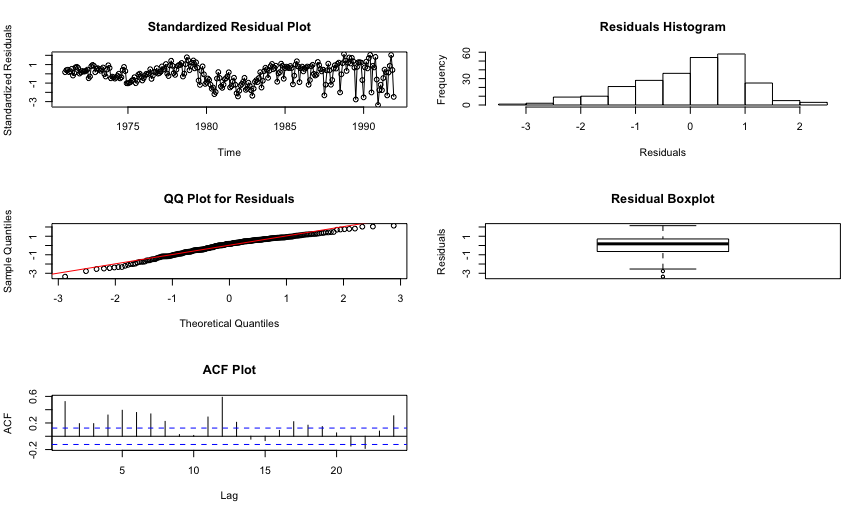
\includegraphics[width=\linewidth]{Images/P3/LFit_Res_Veh.png}
    \caption[Residual diagnostics of the harmonic fit over the original Vehicles data.]{Residual diagnostics of the harmonic fit over the original Vehicles data. Here, we again see the non-normality of the residuals.}
    \label{fig:res_veh_har}
\end{figure}
Furthermore, we check the AIC and BIC values along with the p-values of the normality checks. Both the normality checks suggest that the residuals are from a non-normal distribution. 
\small\begin{block}
Original Chemicals Data

Shapiro-Wilk normality test
W = 0.98358, p-value = 0.005282

Exact runs test
Runs = 56, p-value < 2.2e-16
alternative hypothesis: two.sided

> AIC(chemicals.fit)
[1] 790.5797
> BIC(chemicals.fit)
[1] 808.2269

Original Vehicles Data

Shapiro-Wilk normality test
W = 0.98358, p-value = 0.005282

Exact runs test
Runs = 56, p-value < 2.2e-16
alternative hypothesis: two.sided

> AIC(vehicles.fit)
[1] 1112.108
> BIC(vehicles.fit)
[1] 1129.755
\end{block}
\normalsize Now, we observe the ACF, PACF, EACF, and ARMA Subset Plots for the detrended data.
\begin{figure}[!htb]
    \centering
    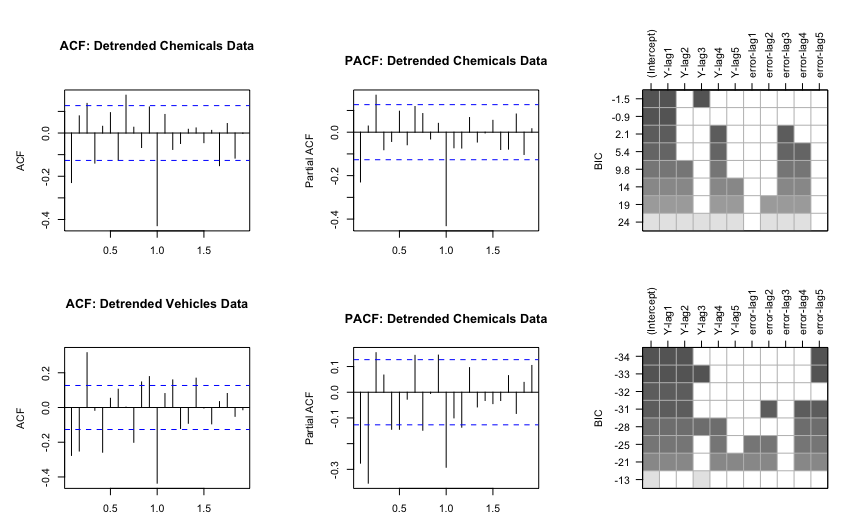
\includegraphics[width=\linewidth]{Images/P3/ACFs_Detrended.png}
    \caption[ACF, PACF, and ARMA subset plots for the detrended Chemicals and Vehicles data.]{ACF, PACF, and ARMA subset plots for the detrended Chemicals and Vehicles data. These show that the detrended data could possible have both AR and MA parts.}
    \label{fig:acf_det}
\end{figure}
The EACF matrices for these data are given below.
\small\begin{block}
> eacf(chemicals.diff2)
AR/MA
  0 1 2 3 4 5 6 7 8 9 10 11 12 13
0 x o x x o o o x o o o  x  o  o 
1 o o x o o o o x o o o  x  o  o 
2 x x o o o o o x o o o  x  o  x 
3 x x x o o o o o o o o  x  o  x 
4 x x o o o o o o o o o  x  o  x 
5 x x o o o o o o o o o  x  x  o 
6 x x o x x o o o o o o  x  o  o 
7 x x x x o o o o o o o  x  o  o 

> eacf(vehicles.diff2)
AR/MA
  0 1 2 3 4 5 6 7 8 9 10 11 12 13
0 x x x o x o o o x x x  x  o  x 
1 x x x o x o o o x o o  x  x  x 
2 x x o x x o o o o o o  x  o  x 
3 x x x o x o o o o o o  x  x  x 
4 x x o o o o o o o o o  x  x  x 
5 x x x o x o o o o o o  x  x  o 
6 x x o x x o o o o o o  x  x  o 
7 x x o o o o o o o o o  x  x  o 
\end{block}
\normalsize Next, we fit the best ARIMA model using the auto.arima function in R and perform the necessary residual diagnostics (using tsdiag function). These are shown in Figures \ref{fig:tsdiag_chem} and \ref{fig:tsdiag_veh}.
\small\begin{block}
> chemicals.arima = auto.arima(chemicals.diff2)
> chemicals.arima
Series: chemicals.diff2 
ARIMA(2,0,2)(0,0,1)[12] with zero mean 

Coefficients:
          ar1      ar2     ma1     ma2     sma1
      -0.9289  -0.8776  0.7277  0.7503  -0.6089
s.e.   0.0644   0.0712  0.0901  0.0911   0.0583

sigma^2 estimated as 0.1409:  log likelihood=-104.97
AIC=221.95   AICc=222.31   BIC=242.8

> vehicles.arima = auto.arima(vehicles.diff2)
> vehicles.arima
Series: vehicles.diff2 
ARIMA(2,0,2)(0,0,1)[12] with zero mean 

Coefficients:
          ar1      ar2     ma1     ma2     sma1
      -0.4311  -0.7637  0.1581  0.5965  -0.5006
s.e.   0.0943   0.1128  0.1040  0.1725   0.0623

sigma^2 estimated as 1.259:  log likelihood=-366.3
AIC=744.61   AICc=744.97   BIC=765.47
\end{block}
\normalsize 
\begin{figure}[!htb]
    \centering
    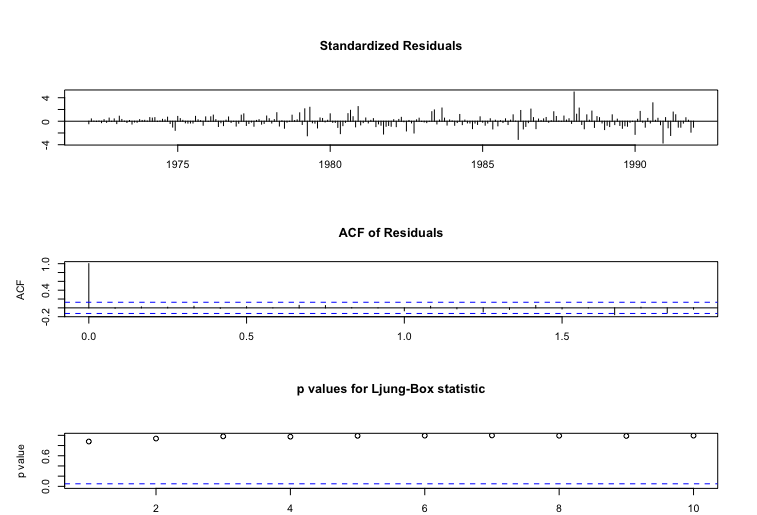
\includegraphics[width=\linewidth]{Images/P3/TSDiag_Chemicals.png}
    \caption[Residual diagnostics for the the ARIMA fit over the detrended Chemicals data.]{Residual diagnostics for the ARIMA fit over the detrended Chemicals data. These show that the residuals closely follow a normal distribution. Also, we observe that the AIC and BIC values have significantly reduced as compared to the harmonic fit over the same data.}
    \label{fig:tsdiag_chem}
\end{figure}

\begin{figure}[!htb]
    \centering
    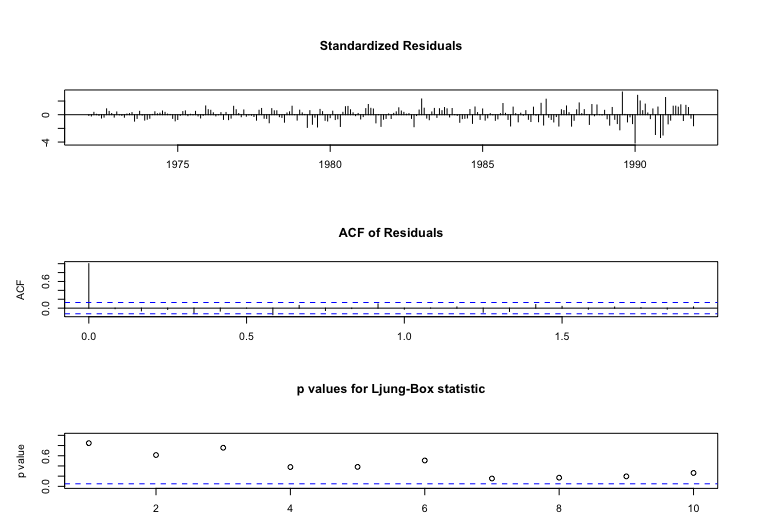
\includegraphics[width=\linewidth]{Images/P3/TSDiag_Veh.png}
    \caption[Residual diagnostics for the the ARIMA fit over the detrended Vehicles data.]{Residual diagnostics for the ARIMA fit over the detrended Vehicles data. These show that the residuals do not closely follow a normal distribution. But, we observe that the AIC and BIC values have significantly reduced as compared to the harmonic fit over the same data.}
    \label{fig:tsdiag_veh}
\end{figure}

Like before, we carry out the normality tests which align with our graphically interpreted results.
\small\begin{block}
Detrended Chemicals Data

Shapiro-Wilk normality test
W = 0.95342, p-value = 5.817e-07

Exact runs test
Runs = 121, p-value = 0.8969
alternative hypothesis: two.sided

Detrended Vehicles Data

Shapiro-Wilk normality test
W = 0.97736, p-value = 0.0007176

Exact runs test
Runs = 109, p-value = 0.1537
alternative hypothesis: two.sided
\end{block}
\normalsize Once these analyses are done, we apply BoxCox transformation (automatically chosen $\lambda_C \approx 0.19$ and $\lambda_V \approx -0.03$ for Chemicals and Vehicles data respectively) to the original data. We also do the same for the detrended data but in that case we first apply the transformation and then detrend.

The model details of the harmonic fit over the transformed data are given below.
\small\begin{block}
Transformed Chemicals Data

Call:
lm(formula = chemicals.bc.tr ~ (har + time(chemicals.bc.tr)))

Residuals:
     Min       1Q   Median       3Q      Max 
-0.40239 -0.13766 -0.00284  0.12268  0.47168 

Coefficients:
                        Estimate Std. Error t value Pr(>|t|)    
(Intercept)           -2.587e+02  3.716e+00 -69.611  < 2e-16 ***
harcos(2*pi*t)        -1.439e-02  1.607e-02  -0.895    0.371    
harsin(2*pi*t)         6.795e-02  1.608e-02   4.226 3.34e-05 ***
time(chemicals.bc.tr)  1.322e-01  1.875e-03  70.490  < 2e-16 ***
---
Signif. codes:  0 ‘***’ 0.001 ‘**’ 0.01 ‘*’ 0.05 ‘.’ 0.1 ‘ ’ 1

Residual standard error: 0.1803 on 248 degrees of freedom
Multiple R-squared:  0.9525,	Adjusted R-squared:  0.9519 
F-statistic:  1658 on 3 and 248 DF,  p-value: < 2.2e-16

Transformed Vehicles Data
Call:
lm(formula = vehicles.bc.tr ~ (har + time(vehicles.bc.tr)))

Residuals:
     Min       1Q   Median       3Q      Max 
-0.51612 -0.12429  0.02448  0.12732  0.41170 

Coefficients:
                       Estimate Std. Error t value Pr(>|t|)    
(Intercept)          -1.272e+02  3.673e+00 -34.628   <2e-16 ***
harcos(2*pi*t)        2.391e-02  1.588e-02   1.506   0.1334    
harsin(2*pi*t)        4.306e-02  1.589e-02   2.710   0.0072 ** 
time(vehicles.bc.tr)  6.534e-02  1.854e-03  35.250   <2e-16 ***
---
Signif. codes:  0 ‘***’ 0.001 ‘**’ 0.01 ‘*’ 0.05 ‘.’ 0.1 ‘ ’ 1

Residual standard error: 0.1783 on 248 degrees of freedom
Multiple R-squared:  0.834,	Adjusted R-squared:  0.832 
F-statistic: 415.3 on 3 and 248 DF,  p-value: < 2.2e-16
\end{block}
\normalsize
\begin{figure}[!htb]
    \centering
    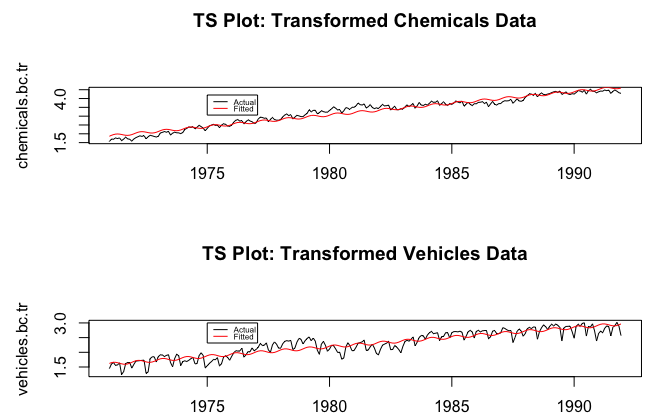
\includegraphics[width=\linewidth]{Images/P3/Lfit_BoxCox.png}
    \caption[Fitting a harmonic model with linear trend over the transformed data.]{Fitting a harmonic model with linear trend over the transformed data. There is not much improvement in the fit as compared to Fig \ref{fig:harmonic_fit}. In fact, the fit over the Chemicals data is worse. Therefore, we do not perform any other diagnostics for this model and carry on with the detrended and stabilized datasets.}
    \label{fig:harmonic_bc_fit}
\end{figure}

Here, in Fig \ref{fig:diff_bc_plots} we observe the temporal patterns of the stabilized datasets (transformed, detrended, and seasonality removed).
\begin{figure}[!htb]
    \centering
    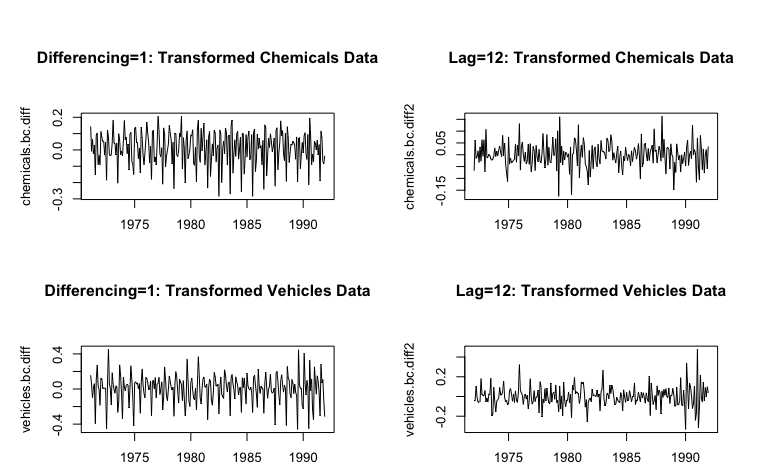
\includegraphics[width=\linewidth]{Images/P3/Diff_BC_Plots.png}
    \caption[Time series plots of the stabilized data.]{Time series plots of the stabilized data. The plots are constructed the same way as in Fig \ref{fig:diff_plots}. However, we see that the stabilized data appears to be more stationary than before.}
    \label{fig:diff_bc_plots}
\end{figure}

Now, we check the different ACF plots depicted in Fig \ref{fig:acf_bc_det}.
\begin{figure}[!htb]
    \centering
    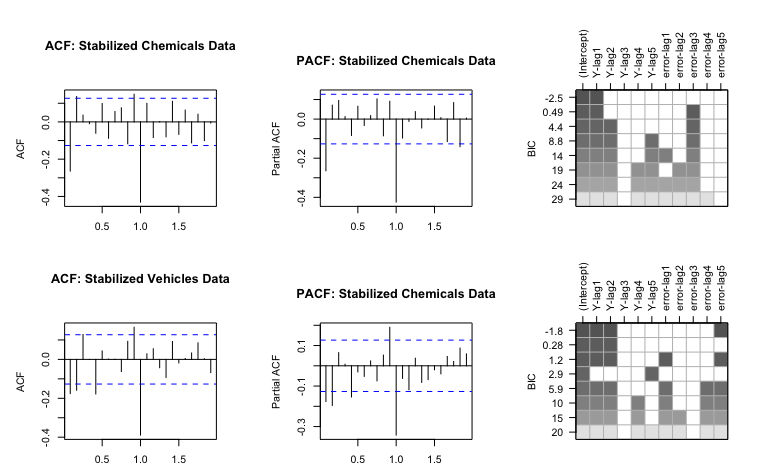
\includegraphics[width=\linewidth]{Images/P3/ACFs_BC_Plots.png}
    \caption[ACF, PACF, and ARMA subset plots for the stabilized Chemicals and Vehicles data.]{ACF, PACF, and ARMA subset plots for the stabilized Chemicals and Vehicles data. These show that the detrended data could possible have both AR and MA parts like before but the AIC and BIC values could be significantly reduced (since $\lambda_C \approx 0.19$ and $\lambda_V \approx -0.03$ for Chemicals and Vehicles data respectively) as compared to Fig \ref{fig:acf_det}.}
    \label{fig:acf_bc_det}
\end{figure}
The EACF matrices for these stabilized datasets are given here.
\small\begin{block}
> eacf(chemicals.bc.diff2)
AR/MA
  0 1 2 3 4 5 6 7 8 9 10 11 12 13
0 x x o o o o o o o o x  x  o  o 
1 x x o o o o o o o o o  x  x  o 
2 x x o o o o o o o o o  x  x  o 
3 o x x o o o o o o o o  x  x  o 
4 x x o o o o o o o o o  x  x  x 
5 x x o o o o o o o o o  x  o  x 
6 x o o o x o o o o o o  x  o  o 
7 x o o x o o o o o o o  x  x  o

> eacf(vehicles.bc.diff2)
AR/MA
  0 1 2 3 4 5 6 7 8 9 10 11 12 13
0 x x o o x o o o o o x  x  o  o 
1 x x o o x o o o o o o  x  x  o 
2 x o o o x o o o o o o  x  x  x 
3 o o x o x o o o o o o  x  x  x 
4 o x x x o o o o o o o  x  x  o 
5 x x x x o o o o o o o  x  x  o 
6 x x o x o o o o o o o  x  x  o 
7 x x o o o o x o o o o  x  o  o 
\end{block}
\normalsize As expected from Fig \ref{fig:acf_bc_det}, we have greatly reduced the AIC and BIC values using transformation. The model details obtained using the auto.arima function are given here. It is noteworthy that, while the number of parameters for the Chemicals data remain the same as before, we have been able to reduce one parameter in case of the Vehicles data. Hence, we do not further check the residuals.
\small\begin{block}
> chemicals.bc.diff2.arima = auto.arima(chemicals.bc.diff2)
> chemicals.bc.diff2.arima

Series: chemicals.bc.diff2 
ARIMA(2,0,2)(0,0,1)[12] with zero mean 

Coefficients:
          ar1      ar2     ma1     ma2     sma1
      -0.9330  -0.9102  0.7469  0.7854  -0.6996
s.e.   0.0548   0.0595  0.0850  0.0741   0.0641

sigma^2 estimated as 0.001787:  log likelihood=415.93
AIC=-819.86   AICc=-819.5   BIC=-799.01

> vehicles.bc.diff2.arima = auto.arima(vehicles.bc.diff2)
> vehicles.bc.diff2.arima

Series: vehicles.bc.diff2 
ARIMA(0,0,2)(0,0,2)[12] with zero mean 

Coefficients:
          ma1      ma2     sma1     sma2
      -0.2106  -0.1494  -0.6332  -0.1205
s.e.   0.0676   0.0740   0.0678   0.0723

sigma^2 estimated as 0.006902:  log likelihood=252.91
AIC=-495.82   AICc=-495.56   BIC=-478.44
\end{block}

\normalsize Therefore, from the above results, it can be concluded that transformation improves the fit of these models. In order to check the cross-correlation between the Chemicals and Vehicles data, we use the ccf function in R (Fig \ref{fig:ccf}). This shows that the sales of chemicals and vehicles are positively correlated. 

\begin{figure}[!htb]
    \centering
    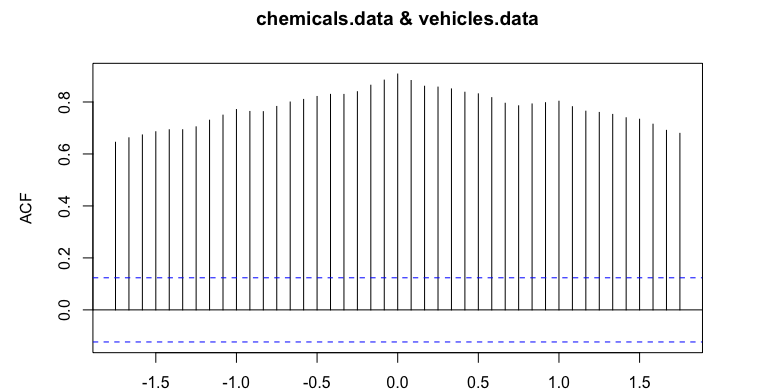
\includegraphics[width=\linewidth]{Images/P3/CCF.png}
    \caption[Cross-correlation plot of Chemicals and Vehicles data.]{Cross-correlation plot of Chemicals and Vehicles data.}
    \label{fig:ccf}
\end{figure}

\item The strong positive correlation between the Chemicals and Vehicles data could be attributed to the increase of vehicle usage over time thereby necessitating more use of chemicals not only for vehicle parts but also for additional utilities like stain removers etc. However, if the month-to-month variation is considered, there are bigger variations in the sales of vehicles. This is because Chemical sales on a monthly basis will not fluctuate much as chemicals are required in a variety of industries. But in case of vehicles, there are additional factors involved such as the economic slowdown which significantly affect the sales.

\end{enumerate}